\documentclass{article}
\usepackage{booktabs}
\renewcommand{\baselinestretch}{1.1}
\usepackage{amsthm,amsmath, amssymb, amsfonts, amscd, xspace, pifont, color}
\usepackage{epsfig, psfrag,subfig}
\usepackage{multirow}
\usepackage[top=1in, bottom=1in, left=1in, right=1in]{geometry}
\usepackage{rotating}
\usepackage[round]{natbib}

\newtheorem{Theorem}{Theorem}[section]
\newtheorem{Lemma}[Theorem]{Lemma}

\newcommand{\FF}{\mathcal{F}}
\newcommand{\GG}{\mathcal{G}}
\newcommand{\LL}{\mathcal{L}}
\newcommand{\RR}{\mathbb{R}}
\newcommand{\Y}{\mathbf{Y}}
\newcommand{\X}{\mathbf{X}}
\newcommand{\Q}{\mathbf{Q}}
\newcommand{\HH}{\mathbf{H}}
\newcommand{\V}{\mathbf{V}}
\newcommand{\VV}{\mathbf{V}^{-1}}
\newcommand{\argmax}{\mathop{\arg\max}}
\newcommand{\argmin}{\mathop{\arg\min}}


\begin{document}

    \begin{center}
        \Large{Apply Gene-Trait Similarity Regression with Gene level Interaction to Real Data}
    \end{center}

    \fontsize{11pt}{\baselineskip}\selectfont

    \section{Method}

        \subsection{The Gene-Trait Similarity Model}
         Denote $Y_i$ as the trait value, $X_i$ the $K\times 1$ covariant vector including the intercept term, and  $1\times l_m$ vector $G_{m,i}$ records the number of distinct alleles on the $mth$ marker for $ith$ individual

         For genetic similarity, define $S_{ij}$ to be the genetic similarity between subjects $i$ and $j$ ($i\neq j$). There are many ways to describe the genetic similarity between individuals. Here, two measurements of $S_{ij}$ based on unphased genotype are introduced. One is Average IBS (identical-by-State) method. It defines the genetic similarity between individual $i$ and $j$ as $S^{ave}_{ij}=\frac{1}{M}\sum^M_{m=1}s^{ave}_{m,ij}$, where
         \[ s^{ave}_{m,ij}=\begin{cases}
                1,\quad G_{m,i} \mbox{ and } G_{m,j} \mbox{ share the same allele and both of them are homozygous genotypes} \\
                \frac{1}{2},\quad G_{m,i} \mbox{ and } G_{m,j} \mbox{ share the same alleles and both of them are heterozygote genotypes} \\
                \frac{1}{2},\quad G_{m,i} \mbox{ and } G_{m,j} \mbox{ share only 1 allele and one of them is homozygous genotype} \\
                \frac{1}{4},\quad G_{m,i} \mbox{ and } G_{m,j} \mbox{ share only 1 allele and both of them are heterozygote genotype} \\
                0,\quad \mbox{o.w}
         \end{cases} \]

         Another way to describe the genetic similarity is so called Typical IBS, here the similarity matrix $S^{typ}_{ij}=\frac{1}{M}\sum^M_{m=1}s^{typ}_{m,ij}$ is calculated by
         \[ s^{typ}_{m,ij}=\begin{cases}
                1,\quad G_{m,i} \mbox{ and } G_{m,j} \mbox{ share the same allele(s)}\\
                \frac{1}{2},\quad G_{m,i} \mbox{ and } G_{m,j} \mbox{ share 1 allele} \\
                0,\quad \mbox{o.w}
         \end{cases} \]

         We can see the difference between two measurements is that Typical IBS only consider the similarity between two markers while Average IBS also considers whether the marker is homozygous or not. If the information for the pahsed haplotype is known,  then we can tell whether the alleles from individual $i$ is identical to the one from individual $j$. Since the haplotype is unknown, we can only have a guess. Average IBS takes the average value while Typical IBS treats the two individuals always share the same haplotype. It is also worth to point out that while the marker information is bi-allelic such as SNP data, the result from Typical IBS and Average IBS would be quite similar since $s^{ave}_{m,ij}$ can not take the value $\frac{1}{4}$ for the heterozygote genotypes are always the same.

         The trait similarity between individual $i$ and $j$:$Z_{ij}$is computed by
         \begin{equation*}
            Z_{ij}=(Y_i-\mu_i)(Y_j-\mu_j)
         \end{equation*}
         where we assume $\mu_i=E(Y_i|X_i,G_i)=X_i\gamma$ is the conditional mean of trait with no genotype effect and $\gamma$ is the effect of the covariant.

         Since we need to consider the Gene interaction, 2 Genes, say, Gene A and Gene B are included. Define $S_{AB,ij}=S_{A,ij}\times S_{B,ij}$, the Gene-Trait similarity model considering the interaction is
         \begin{equation}
            E(Z_{ij})=\tau_AS_{A,ij}+\tau_BS_{B,ij}+\phi S_{AB,ij}
         \end{equation}
        By the definition of $Z_{ij}$, it should has zero mean.

        \subsection{The Joint Test}
        The joint test tests the hypothesis $H_{0,1}$: $\tau_A=\tau_B=\phi=0$. It is hard to directly derive the test for the testing based on (1). However, we find the score test by taking advantage of the connection between the similarity model and the variance component model (\cite{Tzeng2009}) which is:
        \begin{equation}
            Y=X\gamma+G_A+G_B+G_{AB}+e
        \end{equation}
        where
        \[G_A   \sim   MN(0, \tau_AS_A)\]
        \[G_B   \sim   MN(0, \tau_BS_B)\]
        \[G_{AB}\sim   MN(0, \phi S_{AB})\]
        \[e     \sim   MN(0,\sigma I)\]

        Simple algebra shows that the score statistic under $H_{0,1}$ is

        \[
            T_1=\frac{1}{2}\Y'P_1S_1P_1\Y
        \]

        where the $P_1=\sigma^{-2}(I-\X(\X'\X)^{-1}\X')=\sigma^{-2}Q$ and $S_1=S_A+S_B+S_{AB}$. It is easy to see that when $H_{0,1}$ is not true, $T_1$ which is as strictly increasing function. Therefore larger values of $T_1$ provides stronger evidence against $H_{0,1}$. This suggests that the testing procedure should be one sided.

        Since Q is projection matrix for $\X$, we can show that
        \[
            T_1=\frac{1}{2\sigma^4}\Y'QS_1Q\Y=\frac{1}{2\sigma^4}(\Y-\X\gamma)'QS_1Q(\Y-\X\gamma)\sim\sum_{i=1}^c\lambda_i\chi^2_1
        \]
        where $\lambda_i$ is the ordered nonezero eigenvalues of matrix $QS_1Q/(2\sigma^2)$

        If $\sigma^2_e$ is unknown, we can replace $\sigma^2_e$ by $\hat{\sigma^2_e}$ using
        \[
            \hat{\sigma^2_e}=\frac{\Y'Q\Y}{N-1}
        \]

        \subsection{The score test for $H_{0,2}$: $\phi=0$}
        If we only want to test the hypothesis for the interaction term, we can also construct a similar score test as the joint test. However, we need to estimate $\tau_A$, $\tau_B$ and $\sigma$ first. Here we use the EM algorithm to get the estimation $\hat{\tau_A}$,$\hat{\tau_B}$ and $\hat{\sigma}$(See Appendix). Based on that, we can use score test $T_2$ for the interaction testing, where
        \[
            T_2=\frac{1}{2}\Y'P_2S_2P_2\Y
        \]
        where $P_2=\VV-\VV\X(\X^T\VV\X)^{-1}\X^T\VV$, $\V=\hat{\tau_A}S_A+\hat{\tau_B}S_B+\hat{\sigma}I$ and $S_2=S_{AB}$. And we can also derive that the distribution of $T_2$ is also a weighted $\chi^2$ distribution, that is:
        \[
            T_2=\frac{1}{2}\Y'P_2S_2P_2\Y\sim\sum_{i=1}^c\lambda_i\chi^2_1
        \]
        where $\lambda_i$ is the  ordered nonezero eigenvalues of matrix $\V^{-\frac{1}{2}}P_2S_2P_2\V^{-\frac{1}{2}}$.

        \subsection{One Gene Test adjust with the other Gene}

        Here we construct the score test for the genetic main effect of a gene conditional on the effect of other gene. This test is performed assuming no gene-gene interactions. This is because in scenarios where the interaction effects do exist, the main effects are typically not well-defined, and its significance depends on the scale of the interacting variables.

        \[
            E(Z_{ij})=\tau_AS_{A,ij}+\tau_BS_{B,ij}
        \]

        Here to test the main effect of Gene A adjusted with Gene B, the corresponding hypothesis is $H_{0,3}$: $\tau_A=0$ (vice versa for the Gene B main effect test). Similar to previous two tests, the following score test can be applied:

        \[
            T_3=\frac{1}{2}\Y'P_3S_3P_3\Y
        \]
        where $P_3=\VV_B-\VV_B\X(\X^T\VV_B\X)^{-1}\X^T\VV_B$, $\V_B=\hat{\tau_B}S^B+\hat{\sigma}I$ and $P_3=S_A$, and we can also derive that the distribution of $T_{OneGene}$ is also weighted $\chi^2$ distribution, that is:
        \[
            T_3=\frac{1}{2}\Y'P_3S_3P_3\Y\sim\sum_{i=1}^c\lambda_i\chi^2_1
        \]
        where $\lambda_i$ is the  ordered nonezero eigenvalues of matrix $\V_B^{-\frac{1}{2}}P_3S_3P_3\V_B^{-\frac{1}{2}}$.

    \section{Simulation study}
        \subsection{Design for Simulation Study}

        We studied the performance of our method and other methods using simulated data.
        % Introduce the other methods:
        Here PCA (Principal Component Analysis) PLS (Partial Least-Square) and simple linear regression are used as bench-marker to jointly test the main effect and the epistasis effect. Only simple Linear regression is applied to compare with our method in epistasis test and one gene test adjust with the other gene.
        % Introduce the two genes involved in the model
        We assume that the true risk model involves causal SNPs located in two genes, Gene A and Gene B. To simulate a realistic LD pattern among the markers, we used real genotype data on Gene RBJ and Gene GPRC5B, two candidate for BMI. Figure 1 shows the LD pattern of the two genes.

        \begin{figure}[htbp]
            \centering
            \subfloat[Gene RBJ]{
                \centering
                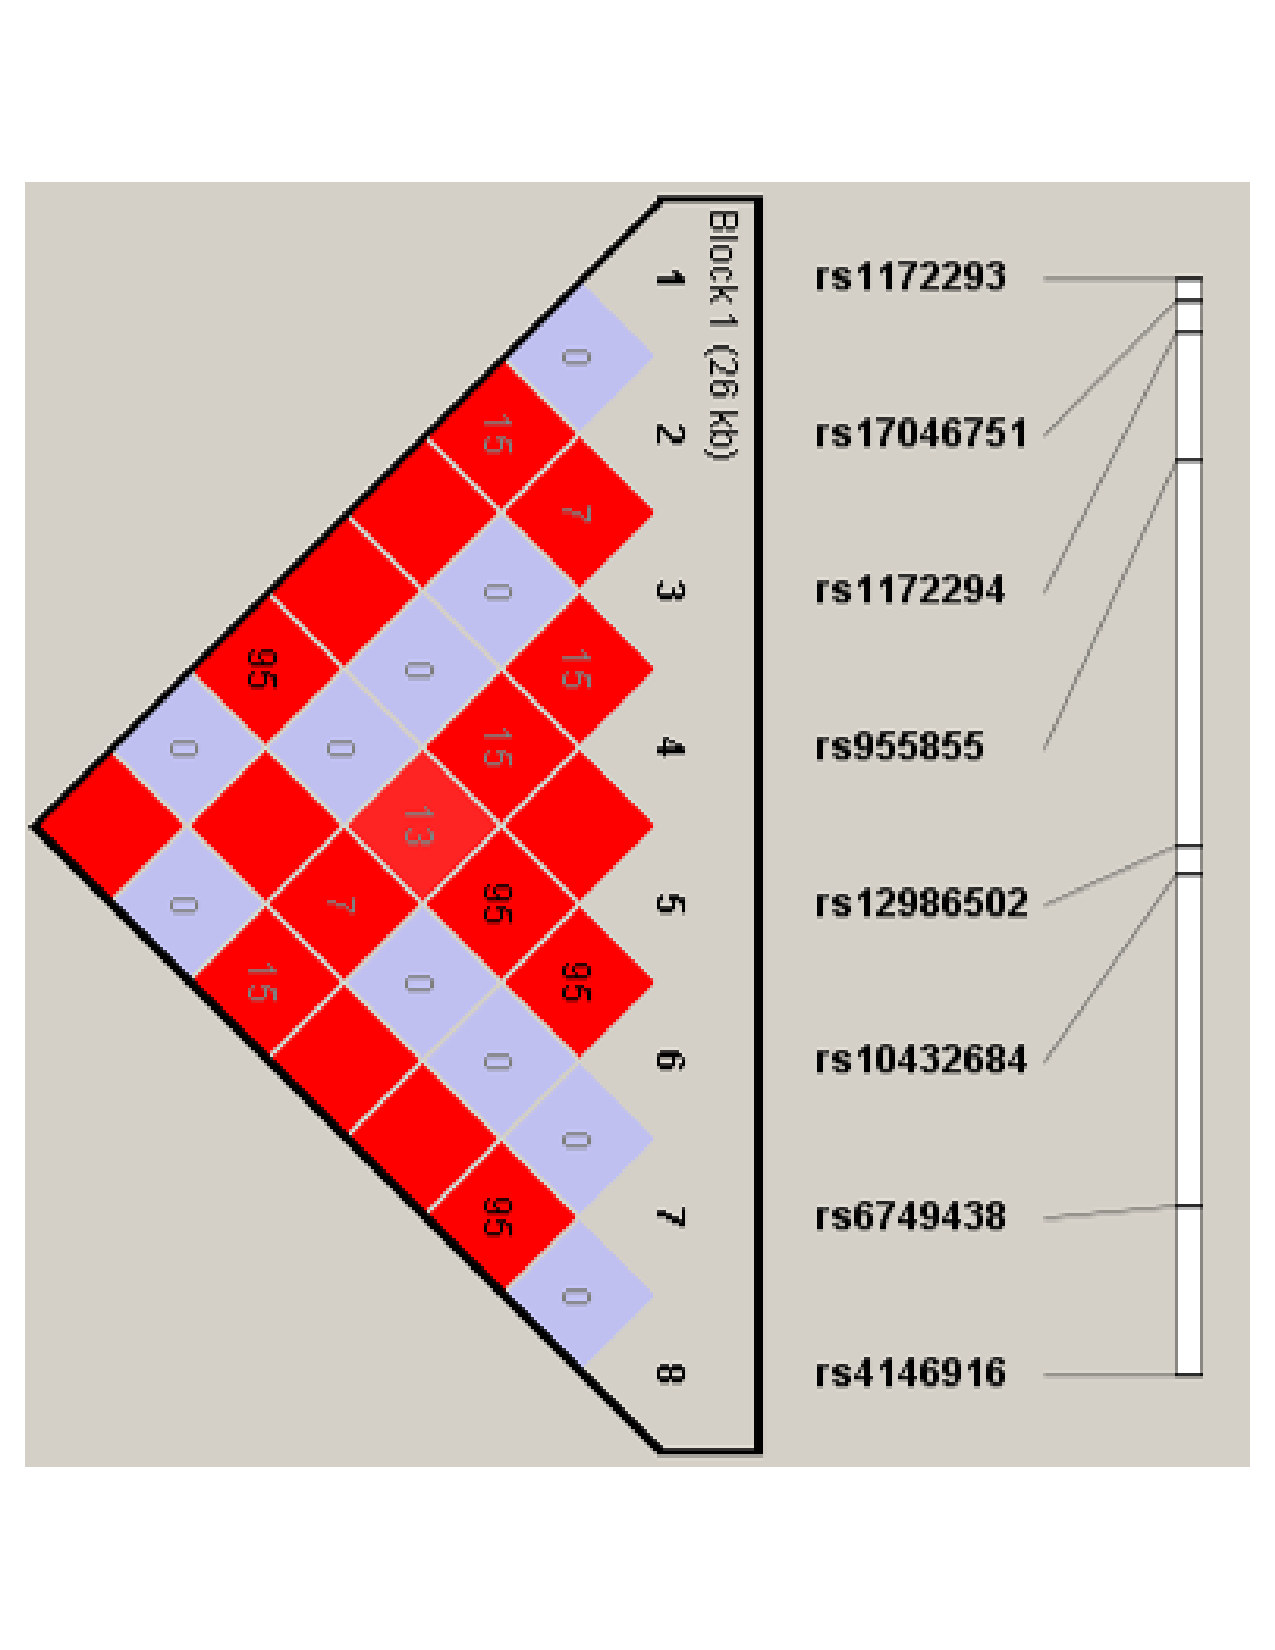
\includegraphics[height=170pt]{RBJ.jpg}

            }
            \hspace{10pt}
            \subfloat[Gene GPRC5B]{
                \centering
                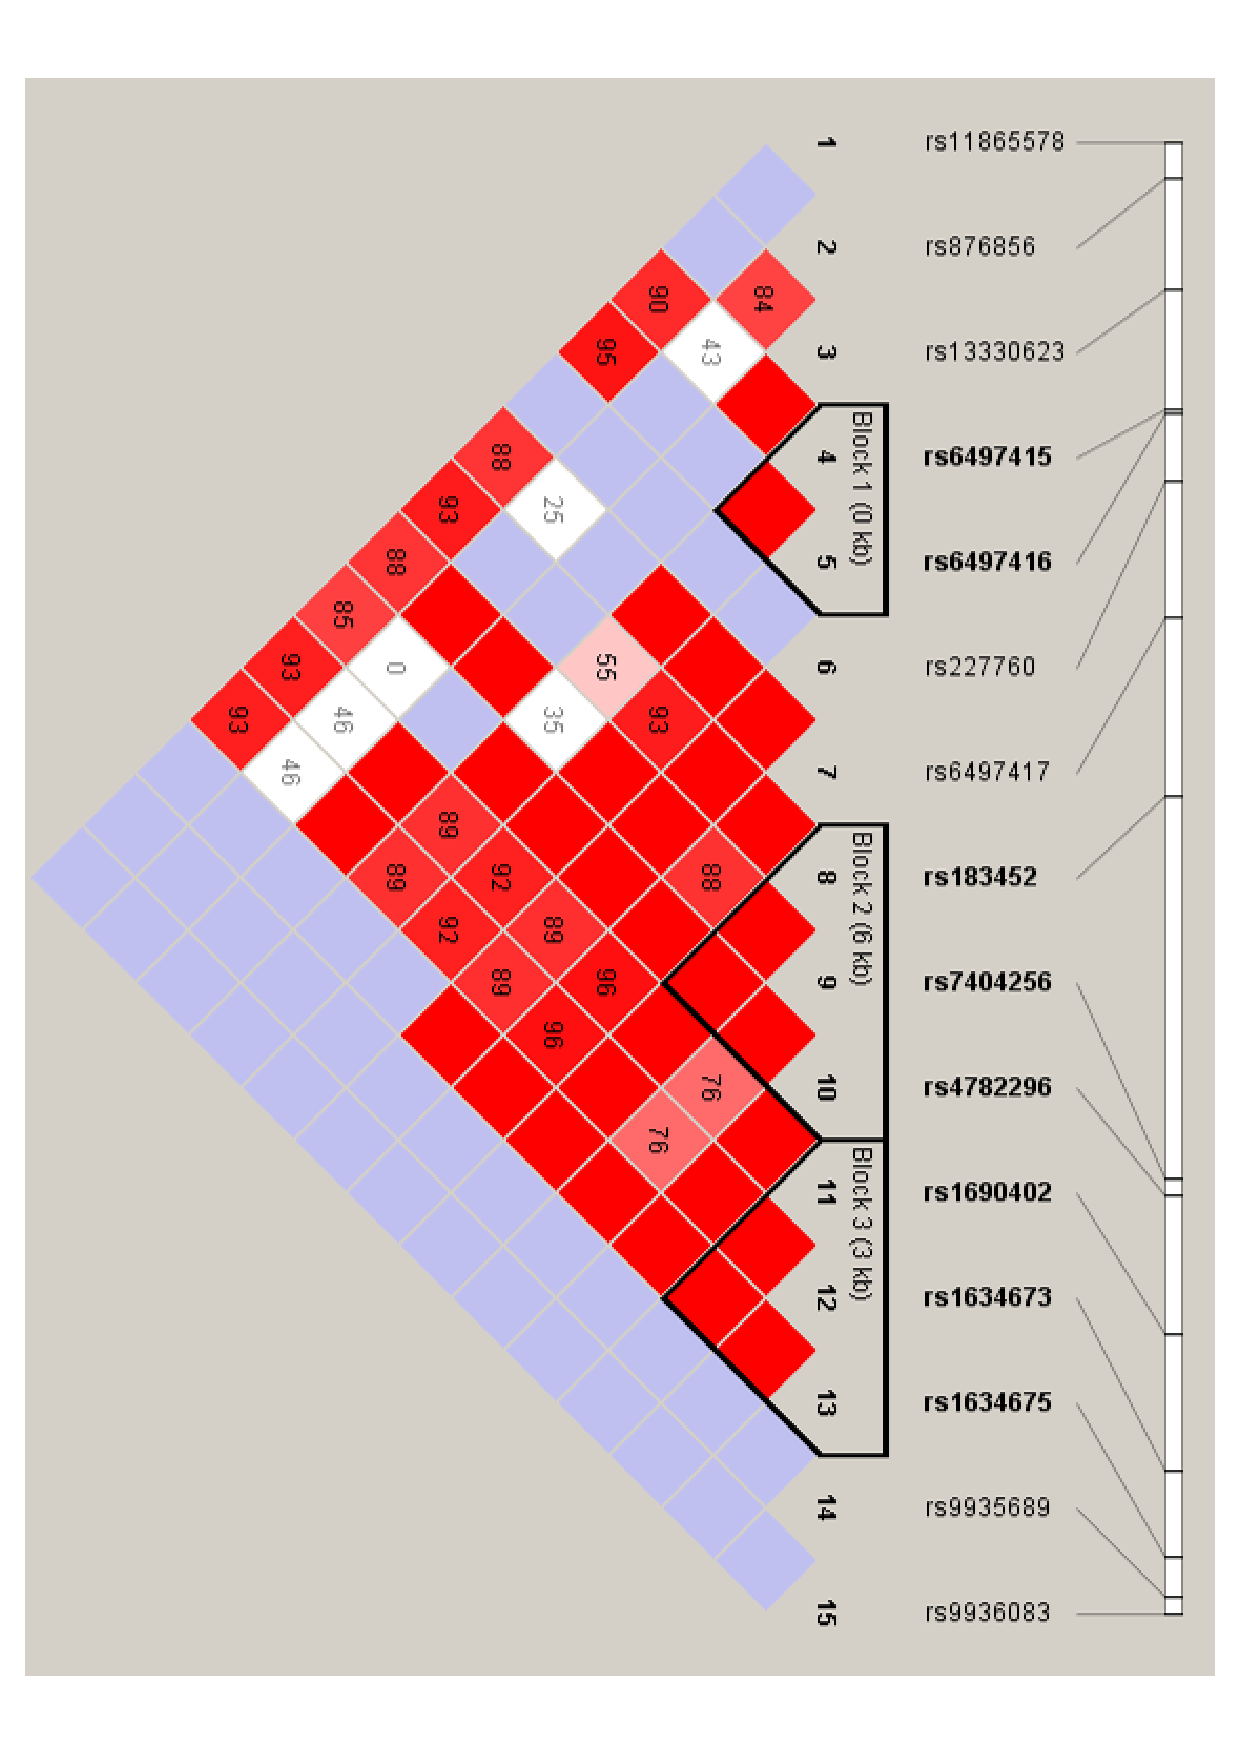
\includegraphics[height=170pt]{GPRC5B.jpg}
            }
            \caption{LD patten of the two genes}
        \end{figure}

        \begin{table}[htbp]
            \centering
            \caption{LD and MAF information for Gene RBJ and GPRC5B}
            \subfloat[Gene RBJ]{
                \begin{minipage}[b]{0.4 \textwidth}
                    \begin{tabular}{c|cc}
                        \toprule
                        SNP	&	LD			&	MAF			\\
                        \midrule
                        1	&	0.588	(	H	)&	0.115	(	M	)\\
                        2	&	0.159	(	L	)&	0.062	(	R	)\\
                        3	&	0.126	(	L	)&	0.482	(	C	)\\
                        4	&	0.588	(	H	)&	0.115	(	M	)\\
                        5	&	0.588	(	H	)&	0.115	(	M	)\\
                        6	&	0.565	(	H	)&	0.119	(	M	)\\
                        7	&	0.159	(	L	)&	0.062	(	R	)\\
                        8	&	0.588	(	H	)&	0.115	(	M	)\\
                        \bottomrule
                    \end{tabular}
                \end{minipage}
            }
            \hspace{10pt}
            \subfloat[Gene GPRC5B]{
                \begin{minipage}[b]{0.4 \textwidth}
                    \begin{tabular}{c|cc}
                        \toprule
                        SNP	&	LD			&	MAF			\\
                        \midrule
                        1	&	0.186	(	N	)&	0.146	(	M	)\\
                        2	&	0.05	(	L	)&	0.066	(	R	)\\
                        3	&	0.065	(	L	)&	0.044	(	R	)\\
                        4	&	0.194	(	N	)&	0.195	(	M	)\\
                        5	&	0.197	(	N	)&	0.143	(	M	)\\
                        6	&	0.136	(	L	)&	0.159	(	M	)\\
                        7	&	0.259	(	H	)&	0.46	(	C	)\\
                        8	&	0.262	(	H	)&	0.336	(	C	)\\
                        9	&	0.23	(	N	)&	0.482	(	C	)\\
                        10	&	0.206	(	N	)&	0.371	(	C	)\\
                        11	&	0.285	(	H	)&	0.394	(	C	)\\
                        12	&	0.285	(	H	)&	0.394	(	C	)\\
                        13	&	0.138	(	L	)&	0.155	(	M	)\\
                        14	&	0	(	L	)&	0.004	(	R	)\\
                        15	&	0	(	L	)&	0.005	(	R	)\\
                        \bottomrule
                    \end{tabular}
                \end{minipage}
            }
        \end{table}

        Table 1 is a brief summary of the two genes. For gene RBJ, it has 8 SNPs, the left table shows the SNPs feature in RBJ. The right table shows the information for SNP in Gene GPRC5B which has 15 SNPs. For each SNP, two measurements are listed. One is the LD pattern, which shows the average correlation between one SNP and other SNPs in the same gene. The other measurement is minor allele freq (MAF). The reason that we focus on LD and MAF is that we think these two would be the main factors affecting the final result. To convince our result analysis, I transform the original quantitative LD and MAF data into categorical data: SNP is defined to have high LD (H) with other SNPs if its average LD $>$ 0.25, if its LD is between 0.18 and 0.25, it is defined as a normal LD. A SNP labeled with C mean it is a common SNP whose MAF $>0.3$,  R means its MAF $\leq 0.1$, and if its MAF is between 0.1 and 0.3, it is labeled as Median (M)

        % Introduce the model
        The trait of each individual in the sample is simulated based on the model listed below according to different purpose.
        \begin{table}[htbp]
            \centering
            \caption{Simulation models}
            \begin{tabular}{c|l}
                \toprule
                \multicolumn{2}{c}{Type I error}\\
                 Model 1 & $Y = \theta_1SNP^A_1+\theta_2SNP^B_1+\theta_{12}SNP^A_1\times SNP^B_1 +e$\\
                \midrule
                \multicolumn{2}{c}{Power}\\
                Model 2 & $Y =\beta\times (SNP^A_1\times SNP^B_1+SNP^A_2\times SNP^B_2)+e$  \\
                Model 3 & $Y =\beta\times (SNP^A_1+SNP^B_1)+e$\\
                Model 4 & $Y =\beta\times (SNP^A_1\times SNP^A_2+SNP^B_1\times SNP^B_2)+e$\\
                \bottomrule
            \end{tabular}
        \end{table}
        $SNP^A_1$, $SNP^A_2$,$SNP^B_1$,$SNP^B_2$ are indicator variables for causal SNPs and $e$ is a normal distributed variable with mean 0 and variance 1. To generate the simulated data, we first download the genotype of RBJ and GPRC5B from HapMap(http://hapmap.ncbi.nlm.nih.gov/) as a gene bank. For the $ith$ individual, we assume no LD between the two genes so we pick RBJ and GPRC5B genotypes from two random sampled persons in the gene bank and combine them together as the $ith$ individual's genotype . We then picked one or two SNPs to generate the phenotype according to different model.

        %for the Type I error.
        The Type I error rate is tested mainly based on Model 1. To simplify the computation, in Type I error rate evaluation, $SNP^A_1$ is the first SNP in Gene A and $SNP^B_1$ is the first SNP in Gene B. For joint test, we set $\theta_1=\theta_2=\theta_{12}=0$. For Epistasis test, we consider 3 situations: (1) neither Gene A or Gene B is associated with the trait($\theta_1=\theta_2=\theta_{12}=0$); (2) Gene A has a main effect to the trait ($\theta_1\neq0,\theta_2=\theta_{12}=0$); (3) both Gene A and Gene B have main effect to the trait, but there is no epitasis effect ($\theta_1\neq0,\theta_2\neq0,\theta_{12}=0$). Similar to the epitasis test, for one gene test, we consider two cases: (1) neither Gene A or Gene B is associated with the trait($\theta_1=\theta_2=\theta_{12}=0$); (2) Gene A has a main effect to the trait ($\theta_1\neq0,\theta_2=\theta_{12}=0$); For each scenario, we run the simulation for 1,000 times with sample 300 to compute the type I error.

        %Design for the power
        To evaluate the power between different methods, we consider three different genetic models(Model 2-4). However, different from Type I error rate evaluation, $SNP^A_1$, $SNP^A_2$, $SNP^B_1$, $SNP^B_2$ are not fixed SNP in corresponding genes. Instead, we try all possible SNP combination sets to test the performance of each methods under different LD and MAF conditions. Model 2 is a typical interaction model which does not contain main effects and the interaction only occurs between Gene A and Gene B. In the pure main effect model 3, there is no epistasis effect. For Model 4, we consider a pure epistasis case where the interaction only occur within genes.We tune $\beta$ so that the power of different SNP sets are distinguishable.

        \subsection{Simulation result: Type I error rate}
        Table 3 shows the result for type I error rate for all the methods at a significance level of $\alpha=0.05$. All methods seems work well in all different settings.

        \begin{table}[htbp]

            \caption{The type I error rate for different test at significance level 0.05}
            \subfloat[Joint test]{
                \begin{minipage}[b]{0.25 \textwidth}
                    \begin{tabular}{c|c}
                        \toprule
                        \multirow{2}*{Method} & $(\theta_1,\theta_2,\theta_{12})$\\
                        \cmidrule{2-2}
                        	&	(0,0,0)		\\
                        \midrule
                        Typical & 0.049\\
                        Average & 0.051\\
                        PCA     & 0.052\\
                        PLS     & 0.051\\
                        LM      & 0.048\\
                        \bottomrule
                    \end{tabular}
                \end{minipage}
            }
            \hspace{10pt}
            \subfloat[Epistasis test]{
                \begin{minipage}[b]{0.37 \textwidth}
                    \begin{tabular}{c|ccc}
                        \toprule
                        \multirow{2}*{Method} & \multicolumn{3}{c}{$(\theta_1,\theta_2,\theta_{12})$}\\
                        \cmidrule{2-4}
                        	&	(0,0,0)	& (2,0,0) & (2,2,0)	\\
                        \midrule
                        Typical & & &0.046\\
                        Average & & &0.050\\
                        LM & 0.052& 0.053& 0.051\\
                        \bottomrule
                    \end{tabular}
                \end{minipage}
            }
            \hspace{10pt}
            \subfloat[One gene test]{
                \begin{minipage}[b]{0.30\textwidth}
                    \begin{tabular}{c|cc}
                        \toprule
                        \multirow{2}*{Method} & \multicolumn{2}{c}{$(\theta_1,\theta_2)$}\\
                        \cmidrule{2-3}
                        	&	(0,0)	& (2,0)\\
                        \midrule
                        Typical &0.045 &0.047\\
                        Average &0.046 &0.049\\
                        LM &0.046 & 0.047\\
                        \bottomrule
                    \end{tabular}
                \end{minipage}
            }
        \end{table}

        \subsection{Simulation result: Power}
        % For model 1:

            % which one is the best?

            % which one is second and so on?

            % Can you explain the reason why they are different?

            % Is there anything else need to mention in model 1?

        % For model 2:

            % which one is the best?

            % which one is second and so on?

            % Can you explain the reason why they are different?

            % Is there anything else need to mention in model 2?

        % For model 3:

            % which one is the best?

            % which one is second and so on?

            % Can you explain the reason why they are different?

            % Is there anything else need to mention in model 1?


    \section{Real Data Analysis}

    % Introduce the Warfarin Data (More information about the Warfarin data is needed here.)

    We have conducted a genetic study with the Warfarin data. In this data set, 2 genes are involved, the first gene contains 7 SNPs and the second gene is a multi-allelic marker which has 6 different genotype. This study involves 301 individuals and records their "ydose"(\textcolor{red}{what is the name of the trait?}). Also available are 6 covariant (e.g. gender, age, race) for each individuals in the study. 
    
    our method and other proposed approaches are applied to find the association between the trait and the two genes using different tests. Table 4 shows the p value for different analysis approaches to locate the association between trait and candidate genes with the covariant. From this table we can see that all methods show significant association between trait and the two genes. But our method show a stronger evidence of association than the other approaches. This result shows us an example of how to improve the power of finding the association even when the interaction is not statistical significant. The real data analysis also suggests us that our method is more powerful than other proposed methods which is consistent with the result we concluded in our simulation study.
    
    \begin{table}[htbp]
        \centering
        \caption{The P-values of different approaches in analysis Warfarin data}
        \begin{tabular}{c|cccc}
            \toprule
            \multirow{2}{*}{Methods} & \multirow{2}{*}{Joint test}& \multirow{2}{*}{Epistasis test} & \multicolumn{2}{c}{One Gene test}\\
            &&&Gene 1&Gene 2\\
            \midrule
             Typical IBS &$5.6\times10^{-20}$ & 0.45 &  $1.67\times 10^{-20}$   &   $1.02\times10^{-7}$ \\
             Average IBS &$5.32\times10^{-21}$ & 0.63 &  $1.44\times 10^{-22}$   &   $9.83\times10^{-9}$  \\
             PCA &$9.48\times10^{-5}$ & - &  -   &   -  \\
             PLS &$9.96\times10^{-5}$ & - &  -   &   -  \\
             LM &$2.2\times10^{-16}$ & 0.844 &  $2.2\times 10^{-16}$   &   $3.23\times10^{-8}$  \\
            \bottomrule
        \end{tabular}
    \end{table}


    \section{Appendix}

        \subsection{Score test for joint test and interaction test}

            For the model:
            \begin{equation*}
                Y=X\gamma+G_A+G_B+G_{AB}+e
            \end{equation*}

            Define $\theta=\{\sigma,\tau_A,\tau_B,\phi\}$, the REML log-likelihood function $L(\theta)$ for the whole data set is:
            \[
                L(\theta)=-\frac{1}{2}\bigg[\log|V|+\log|\X'V^{-1}\X|+\Y'P\Y\bigg]
            \]

             where $V=Var(Y)=\tau_AS_A+\tau_BS_B+\phi S_{AB}+\sigma I$ is the marginal variance of $\Y$ and $P=V^{-1}-V^{-1}\X(\X'V^{-1}\X)^{-1}\X'V^{-1}$ is the projection matrix for the model.

            Simple algebra shows that the score statistic under $H_0:\tau_A=\tau_B=\phi=0$ is

            \[
                U_{\sigma^2_b}=\frac{\partial L(\sigma^2_b,\sigma^2_e)}{\partial \sigma^2_b}\bigg|_{\sigma^2_b=0}=\frac{1}{2}[\Y'P_0SP_0\Y-tr(P_0S)]
            \]

            where the $P_0=\sigma^{-2}_e(I-\X(\X'\X)^{-1}\X')=\sigma^{-2}_eQ$. It is easy seen that $E(U_{\sigma^2_b})=0$ under $H_0^*$ and when $\sigma^2_b>0$, $E(U_{\sigma^2_b})=\sigma^2_b\cdot tr(QSQS)/(2\sigma^4_e)$ which is a strictly increasing function. Therefore larger values of $U_{\sigma_b^2}$ provides stronger evidence against $H_0^*$. This suggests that the testing procedure should be one sided.

            If $\sigma_e^2$ is known, the second term in our test is a constant. Therefore using the score statistic is equivalent to using the first term of $U_{\sigma^2_b}$ (denoted by $T$):
            \[
                T=\frac{1}{2}\Y'P_0SP_0\Y=\frac{1}{2\sigma^4_e}\Y'QSQ\Y
            \]
            Since Q is projection matrix for $\X$, we can show that
            \[
                T=\frac{1}{2\sigma^4_e}\Y'QSQ\Y=\frac{1}{2\sigma^4_e}(\Y-\X\mu)'QSQ(\Y-\X\mu)\sim\sum_{i=1}^c\lambda_i\chi^2_1
            \]
            where $\lambda_i$ is the ordered nonezero eigenvalues of teh matrix $QSQ/(2\sigma^2_e)$

            If $\sigma^2_e$ is unknown, we can replace $\sigma^2_e$ by $\hat{\sigma^2_e}$ using
            \[
                \hat{\sigma^2_e}=\frac{\Y'Q\Y}{N-1}
            \]

        \subsection{EM algorithm to estimate $\tau_A$, $\tau_B$ and $\sigma$}
            The model under the null hypothesis os $\phi=0$ is
            \[
                Y=X\gamma+G_A+G_B+e
            \]

            Y: $N\times1$ matrix, records trait value.

            X: $N\times p$ matrix, records the covariant.

            $\gamma$: $p\times 1$, the effect of covariant.

            $G_A$: the gene effect for Gene A, treated as an random effect. $G_A\sim N(0, \tau_AS_A)$, $S_A$ is the similarity matrix which records the genetic similarity between individuals.

            $G_B$: the gene effect for Gene B, also treated as an random effect. $G_A$ and  $G_B$ are assumed to be independent.

            $e$: $N\times1$ matrix,  the error term. $e\sim N (0, \sigma I)$.

            Define $U=A^TY$ with the restriction that $A^TA=I_{N-p}$ and $AA^T=I-P_X$.

            It is easy to find out that : $E(U)=0$ and $Var(U)=A^TVA$ where $V=Var(Y)=\tau_AS_A+\tau_BS_B+\sigma I$.

            \[ \begin{split}
                Cov(U,G_A)=& Cov(A^TX\gamma+A^TG_A+A^TG_B+A^Te,G_A)\\
                          =& Cov(A^TG_A,G_A)\\
                          =& A^TCov(G_A,G_A)\\
                          =&\tau_AA^TS_A
            \end{split}\]

            In the same way, we have$Cov(U,G_B)=\tau_BA^TS_B$ and $Cov(G_A,G_B)=0$ since they are independent.

            Therefore, the joint distribution of $(U,G_A,G_B)^T$ is
            \[
                \begin{pmatrix} U\\G_A\\G_B \end{pmatrix} \sim MN \begin{pmatrix} \mu=\begin{pmatrix} 0\\0\\0 \end{pmatrix},\quad \Sigma=\begin{pmatrix} A^TVA&\tau_AA^TS_A&\tau_BA^TS_B\\ \tau_AS_AA&\tau_AS_A&0\\\tau_BS_BA&0&\tau_BS_B \end{pmatrix} \end{pmatrix}
            \]

            so we can have the following conditional mean and variance,
            \begin{enumerate}
                \item the conditional mean and variance for $U$ are
                    \[\begin{split}
                        E(U|G_A,G_B)=&A^T(G_A+G_B)\\
                        Var(U|G_A,G_B) = & \sigma I_{N-p}
                    \end{split}\]
                \item the conditional mean and variance for $G_A$, since $Cov(G_A,G_B)=0$
                    \[\begin{split}
                        E(G_A|G_B,U)=&E(G_A|U)\\
                                                   =&\tau_AS_AA(A^TVA)^{-1}A^TY\\
                        Var(G_A|G_B,U)=&Var(G_A|U)\\
                                                       =&\tau_AS_A-\tau_A^2S_AA(A^TVA)^{-1}A^TS_A
                    \end{split}\]
                    Simple algebra shows that $A(A^TVA)^{-1}A^T=P=V^{-1}-V^{-1}X(X^TV^{-1}X)^{-1}X^TV^{-1}$, so that
                    \[\begin{split}
                        E(G_A|G_B,U)=&\tau_AS_APY=g_A\\
                        Var(G_A|G_B,U)=&\tau_AS_A-\tau_A^2S_APS_A=v_A
                    \end{split}\]
                \item Similarly, the conditional mean and variance for $G_B$ are
                     \[\begin{split}
                        E(G_B|G_A,U)=&\tau_BS_BPY=g_B\\
                        Var(G_B|G_A,U)=&\tau_BS_B-\tau_B^2S_BPS_B=v_B
                    \end{split}\]
            \end{enumerate}

            Define $\theta=\{\sigma,\tau_A,\tau_B\}$, according to the EM algorithm, we need to first compute the $\log L(\theta^{(t)}|U,G_A,G_B)$,
            \[\begin{split}
                \log L(\theta^{(t)}|U,G_A,G_B)=&f(U,G_A,G_B|\theta^{(t)})\\
                                                                         =&\log f(U|G_A,G_B,\theta^{(t)})+\log f(G_A|\theta^{(t)})+\log f(G_B|\theta^{(t)})
            \end{split}\]

            Since $S_A$ and $S_B$ are singular, we have,
            \[
                f(G_A)=\dfrac{1}{((2\pi)^{rank(S_A)}|\tau_AS_A|_+)^{\frac{1}{2}}}\exp\Big (-\dfrac{1}{2}G_A^T(\tau_AS_A)^-G_A\Big)
            \]

            where $|\tau_AS_A|_+$ is the Pseudo-Determinant, and $(\tau_AS_A)^-)$ is the Generalized inverse.

            Define $rank(S_A)=q_A$, $rank(S_B)=q_B$, we have,
            \[\begin{split}
                f(G_A)=&\dfrac{1}{((2\pi)^{q_A}\tau_A^{q_A}|S_A|_+)^{\frac{1}{2}}}\exp\Big (-\dfrac{1}{2\tau_A}G_A^T(S_A)^-G_A\Big)\\
                f(G_B)=&\dfrac{1}{((2\pi)^{q_B}\tau_B^{q_B}|S_B|_+)^{\frac{1}{2}}}\exp \Big(-\dfrac{1}{2\tau_B}G_B^T(S_B)^-G_B\Big)
            \end{split}\]

            therefore,

            \[\begin{split}
               \log f(G_A)=&constant -\dfrac{q_A}{2}\log \tau_A-\dfrac{1}{2}\log(|S_A|_+)-\dfrac{1}{2\tau_A}G_A^TS_A^-G_A\\
               \log f(G_B)=&constant -\dfrac{q_B}{2}\log \tau_B-\dfrac{1}{2}\log(|S_B|_+)-\dfrac{1}{2\tau_B}G_B^TS_B^-G_B\\
               \log f(U|G_A,G_B) =& constant-\dfrac{N-p}{2}\log\sigma-\dfrac{1}{2\sigma}\Big[(Y-G_A-G_B)^T(I-P_X)(Y-G_A-G_B)   \Big]
            \end{split}\]

            EM algorithm treats $G_A$ and $G_B$ as missing values. So instead of estimating $G_A$ and $G_B$ and then plugging them into the $\log L$, EM algorithm calculate the expectation of $\log L$ given $U$ and $\theta^{(t-1)}$, then based on $E(\log L|U,\theta^{(t-1)})$, $\theta^{(t)}$ are calculated by taking partial derivative.

            \[
                E\Big(\log L\Big|U,\theta^{(t-1)}\Big)=E\Big(\log f(G_A)\Big|U,\theta^{(t-1)}\Big)+E\Big(\log f(G_B)\Big|U,\theta^{(t-1)}\Big)+E\Big(\log f(U|G_A,G_B)\Big|\theta^{(t-1)}\Big)
            \]

            It is easy to find out that to estimate $\tau_A^{(t)}$, we just need to consider $E\Big(\log f(G_A)\Big|U,\theta^{(t-1)}\Big)$, so let
            \[\frac{\partial E\Big(\log f(G_A)\Big|U,\theta^{(t-1)}\Big)}{\partial\tau_A}=0\]
            we have,
            \[
                -\dfrac{q_A}{2\tau_A}+\dfrac{1}{2\tau_A^2}E\Big(G_A^TS_A^-G_A\Big|U,\theta^{(t-1)}  \Big)=0
            \]

            \[
                E\Big(G_A^TS_A^-G_A\Big|U,\theta^{(t-1)} \Big)=\big(g_A^{(t-1)}\big)^TS_A^-g_A^{(t-1)}+tr(S_A^-v_A^{(t-1)})
            \]
            plugging the expression of $g_A^{(t-1)}$ and $v_A^{(t-1)}$, finally we have
            \[
                \tau_A^{(t)}=\tau_A^{(t-1)}+\dfrac{[\tau_A^{t-1}]^2}{q_A}\Big[Y^TPS_APY-tr(S_AP) \Big]
            \]
            In the same way, we can estimate $\tau_B^{(t)}$ by
            \[
                \tau_B^{(t)}=\tau_B^{(t-1)}+\dfrac{[\tau_B^{t-1}]^2}{q_B}\Big[Y^TPS_BPY-tr(S_BP) \Big]
            \]
            To estimate $\sigma^{(t)}$, we just need to consider $E\Big(\log f(U|G_A,G_B)\Big|\theta^{(t-1)}\Big)$, so the final expression of $\sigma^{(t)}$ is
            \[
                \sigma^{(t)}=\dfrac{1}{N-p}\Big\{\Big[(Y^*)^T(I-P_X)Y^*\Big] + tr\Big[(I-P_X)\Big(\tau_A^{(t-1)}S_A-(\tau_A^{(t-1)})^2S_APS_A+\tau_B^{(t-1)}S_B-(\tau_B^{(t-1)})^2S_BPS_B\Big)\Big]         \Big\}
            \]
        where $Y^*=Y-\tau_A^{(t-1)}S_APY-\tau_B^{(t-1)}S_BPY$
    \bibliographystyle{abbrvnat}
    \bibliography{reflist}

\end{document} 